
\documentclass[xcolor={dvipsnames}]{beamer}
\usetheme{Szeged}
\usecolortheme{seagull}

\usepackage{color}
\usepackage[utf8]{inputenc}
\usepackage[T1]{fontenc}
\usepackage{verbatim}
\usepackage{caption}
%custom packages
\usepackage{amssymb,amsmath}
\usepackage{relsize}

\definecolor{g}{rgb}{0.3,0.61,0.59}


\newcommand\independent{\protect\mathpalette{\protect\independenT}{\perp}}
\def\independenT#1#2{\mathrel{\rlap{$#1#2$}\mkern2mu{#1#2}}}
\newcommand{\trans}{^{\scriptscriptstyle \top}}



%custom commands
\newcommand{\ev}{\mathbb{E}}

%\usepackage[pdftex]{graphicx}

\title{A Wild Bootstrap for Degenerate Kernel Tests}
\author{Kacper Chwialkowski \inst{1} \and Dino Sejdinovic \inst{2} \and Arthur Gretton \inst{2}}
\institute[UCL]{\inst{1} UCL, Computer Science \and %
                      \inst{2} UCL, Gatsby Computational Neuroscience Unit}

\titlegraphic{
    %
\includegraphics[width=2cm]{csml_logo_vector2.pdf}\hspace*{4.75cm}~%
   
\includegraphics[width=2cm]{../img/csml_logo_vector2.pdf}
}
\begin{document}

\frame{\titlepage}

 
\frame{
\begin{columns}[c] 
    \column{.5\textwidth} 
    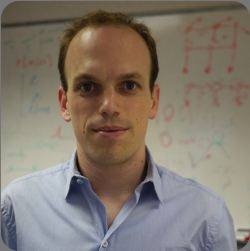
\includegraphics[width=0.5\textheight]{../img/arthur6.jpg}\\
    Arthur
    \column{.5\textwidth}
    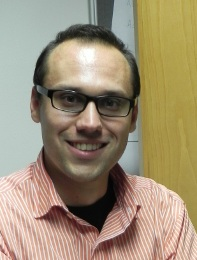
\includegraphics[width=0.5\textheight]{../img/dino.JPG} \\
    Dino
    \end{columns}
}

\section{Introduction}
\frame{
\frametitle{Maximum Mean Discrepancy for Random Processes}
\begin{columns}[c] 
    \column{.8\textwidth} 
    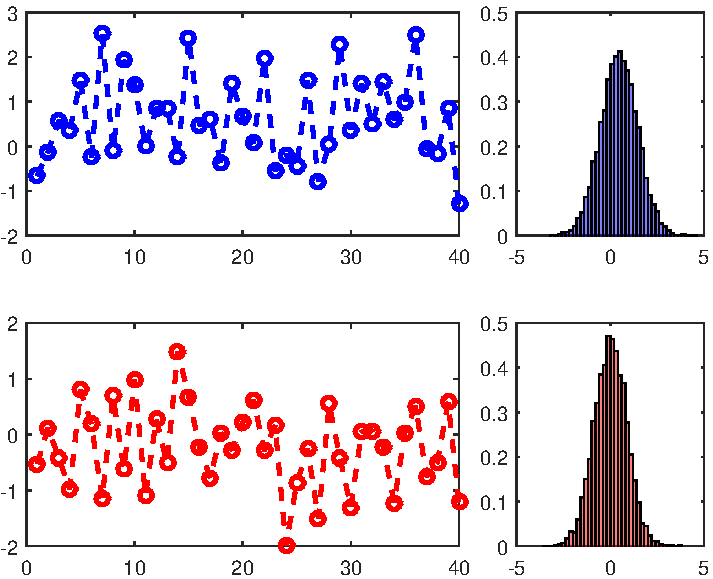
\includegraphics[height=0.8\textheight]{../img/introDep.pdf}
    \column{.2\textwidth}
    Is \\[1em] {\larger[5]$ \color{blue} P$} \\[1em] the same  distribution as  \\[1em]  {\larger[5]$\color{red} Q$} \\[1em] ?
    \end{columns}
}

 
\frame{
\frametitle{Statistical Tests for Random Processes}
Where one can use Maximum Mean Discrepancy ?
\begin{itemize}		
	\item Markov chains diagnostics
	\item Change point detection
\end{itemize}
Other tests
\begin{itemize}		
	\item Hilbert Schmidt Independence Criterion
		\begin{itemize}		
			\item Dependency structure in financial markets 
			\item Brain region activation
		\end{itemize}
	\item Three Variables Interaction 	
\end{itemize}
}


\frame{
\frametitle{Maximum Mean Discrepancy for i.i.d observations}
\begin{columns}[c] 
    \column{.8\textwidth} 
    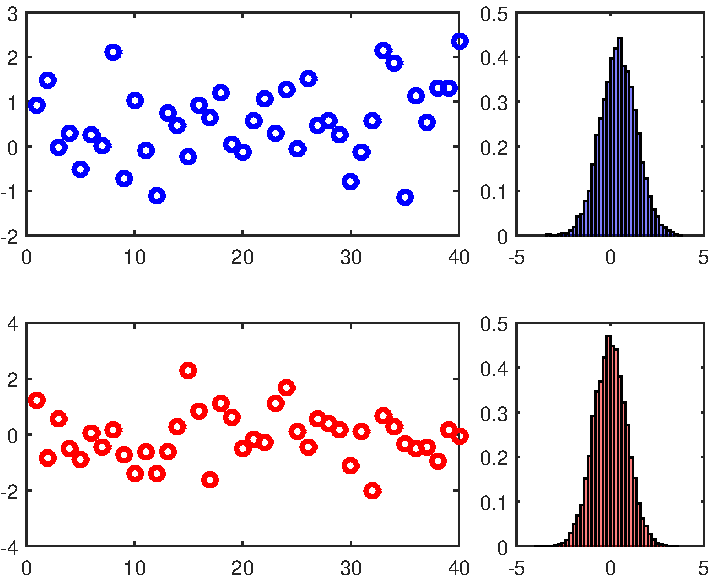
\includegraphics[height=0.8\textheight]{../img/introNoDep.pdf}
    \column{.2\textwidth}
    Is \\[1em] {\larger[5]$ \color{blue} P$} \\[1em] the same  distribution as  \\[1em]  {\larger[5]$\color{red} Q$} \\[1em] ?
    \end{columns}
}

\newcommand{\kpp}{\mathord{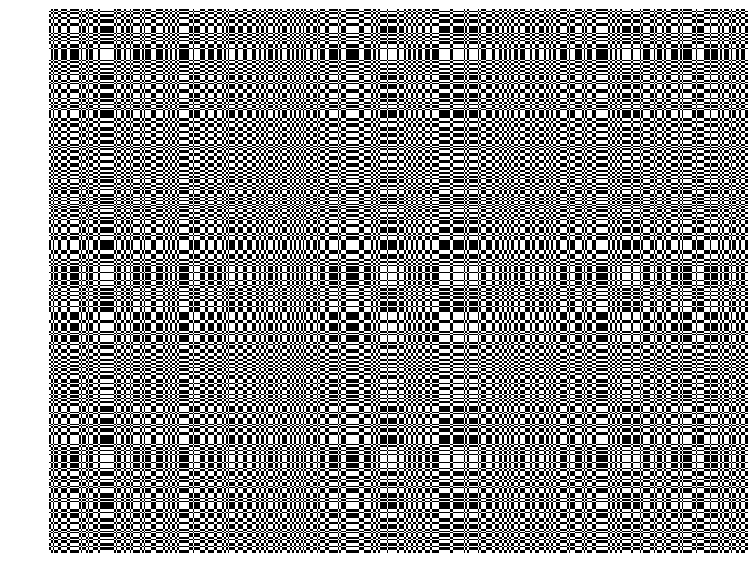
\includegraphics[height=2cm]{../img/KPP.pdf}}}
\newcommand{\kqq}{\mathord{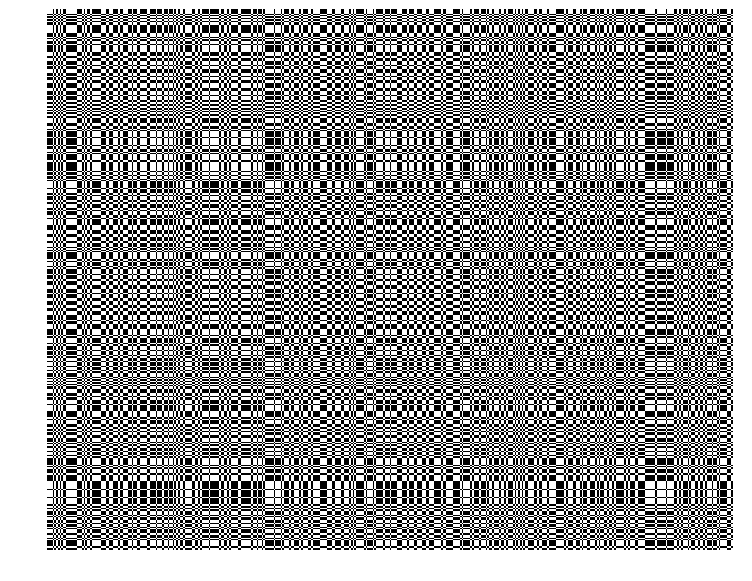
\includegraphics[height=2cm]{../img/KQQ.pdf}}}
\newcommand{\kpq}{\mathord{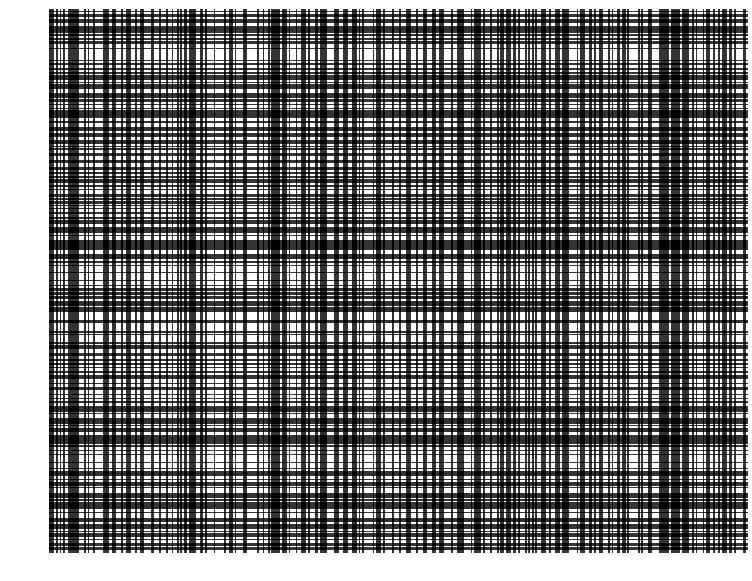
\includegraphics[height=2cm]{../img/KPQ.pdf}}}

\frame{
\frametitle{Similarity}
\begin{align*}
K_{{\color{blue}P,P}}=
\begin{bmatrix}
	k( {\color{blue}X_1},{\color{blue}X_1)} &   \ldots & k({\color{blue}X_1},{\color{blue}X_n})\\
	\vdots &  \ddots & \vdots\\
	k({\color{blue}X_n},{\color{blue}X_1})  &  \ldots & k({\color{blue}X_n},{\color{blue}X_n})
\end{bmatrix} = 
\begin{matrix}
\kpp
\end{matrix}
\\
K_{{\color{red}Q,Q}}=
\begin{bmatrix}
	k({\color{red}Y_1},{\color{red}Y_1)} &   \ldots & k({\color{red}Y_1},{\color{red}Y_n})\\
	\vdots &  \ddots & \vdots\\
	k({\color{red}Y_n},{\color{red}Y_1})  &  \ldots & k({\color{red}Y_n},{\color{red}Y_n})
\end{bmatrix}= 
\begin{matrix}
\kqq
\end{matrix}
\\
K_{{\color{red}P},{\color{blue}Q}}=
\begin{bmatrix}
	k({\color{blue}X_1},{\color{red}Y_1}) &   \ldots & k({\color{blue}X_1},{\color{red}Y_n})\\
	\vdots &  \ddots & \vdots\\
	k({\color{blue}X_n},{\color{red}Y_1})  &  \ldots & k({\color{blue}X_n},{\color{red}Y_n})
\end{bmatrix}=
\begin{matrix}
\kpq
\end{matrix}
\end{align*}
}
\newcommand{\gram}{\mathord{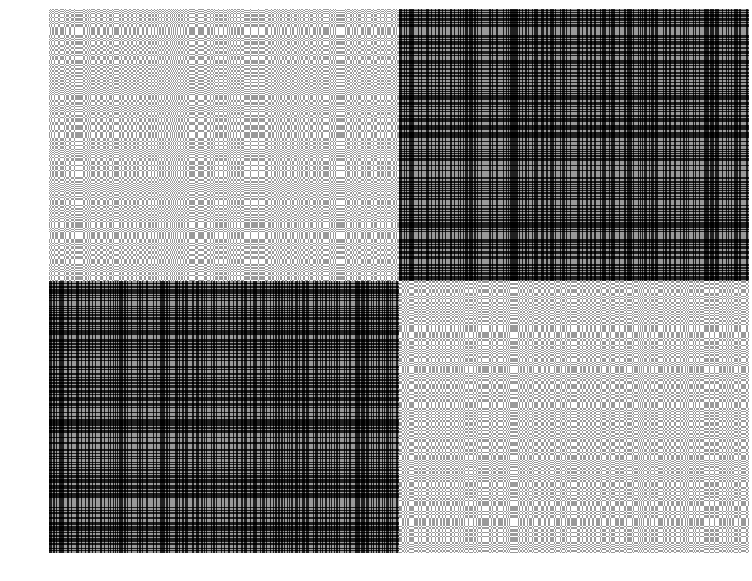
\includegraphics[height=2cm]{../img/Gram.pdf}}}
\newcommand{\gramn}{\mathord{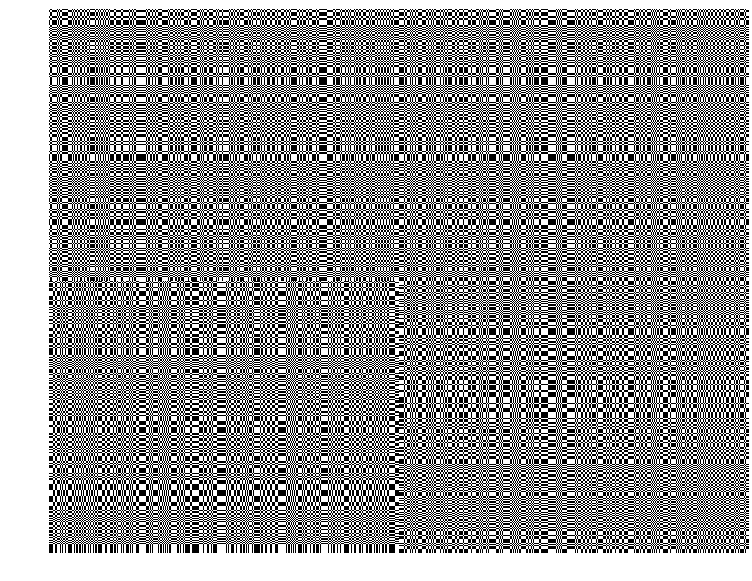
\includegraphics[height=2cm]{../img/Gramn.pdf}}}

\frame{
\frametitle{Similarity}
\begin{align*}
{\color{blue} P} \neq {\color{red} Q} \Rightarrow 
\begin{bmatrix}
	K_{{\color{blue}P,P}}  &   K_{{\color{red}P},{\color{blue}Q}}\\
	K_{{\color{red}Q},{\color{blue}P}}  &  K_{{\color{red}Q,Q}}
\end{bmatrix} = 
\begin{matrix}
\gram
\end{matrix}
\end{align*}
\pause
\begin{align*}
{\color{blue} P }= {\color{red} Q} \Rightarrow
\begin{bmatrix}
	K_{{\color{blue}P,P}}  &   K_{{\color{blue}P,\color{red}Q}}\\
	K_{{\color{red}Q},{\color{blue}P}}  &  K_{{\color{red}Q,Q}}
\end{bmatrix} = 
\begin{matrix}
\gramn
\end{matrix}
\end{align*}
}


\frame{
\frametitle{Quantifying Similarity}
\begin{align*}
 V_n = \overline{ K_{{\color{blue}P,P}}} + \overline{ K_{{\color{red}Q,Q}} } - 2 \overline{  K_{{\color{blue}P,\color{red}Q}} }
\end{align*}
\begin{figure}
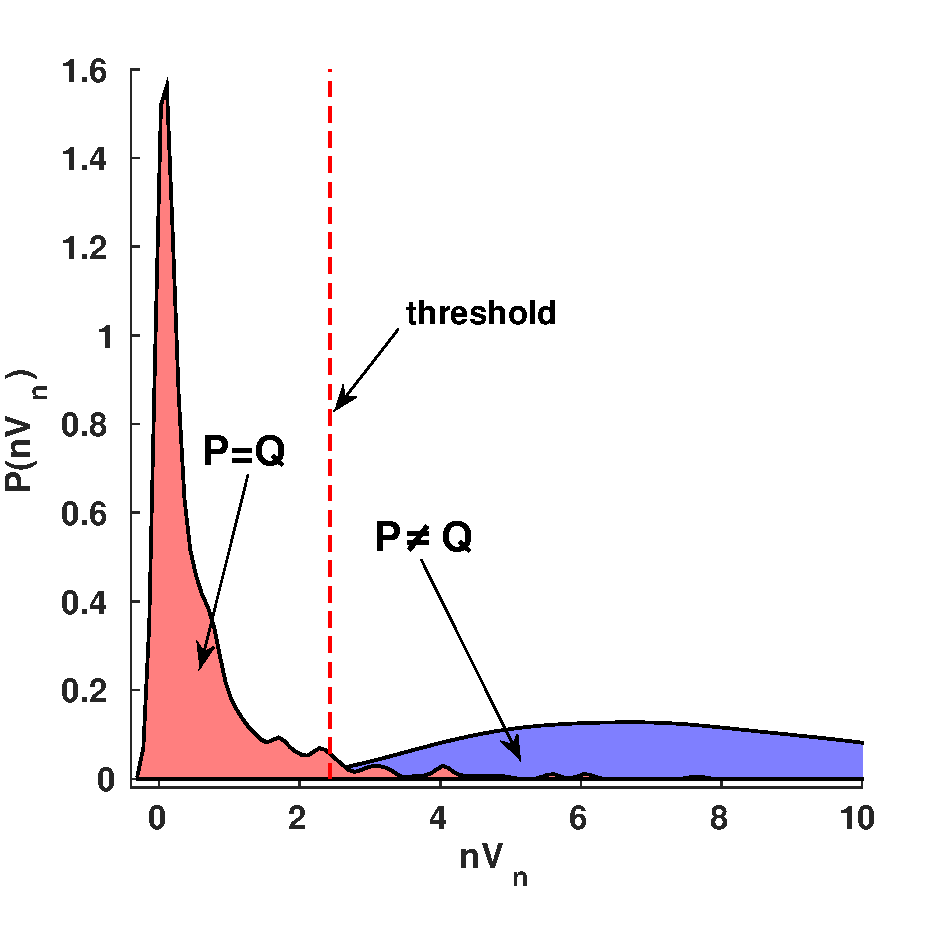
\includegraphics[width=0.55\textwidth]{../img/altAndNull.pdf}

\end{figure}
   
}

\newcommand*{\Scale}[2][4]{\scalebox{#1}{\ensuremath{#2}}}%
\frame{
\frametitle{Putting Hands on $V_n$ Distribution }
$$W= (-1,1,1,\quad \cdots \quad,-1,-1,-1)$$
\begin{align*}
&{\begin{bmatrix}
	K_{{\color{blue}P,P}}  &   K_{{\color{blue}P,\color{red}Q}}\\
	K_{{\color{red}Q},{\color{blue}P}}  &  K_{{\color{red}Q,Q}}
\end{bmatrix} } & \odot
&\begin{bmatrix}
\Scale[2] {W \trans{W}}
\end{bmatrix} &= 
&\begin{bmatrix}
\Scale[2] ?
\end{bmatrix} \\
&\begin{matrix}
\gram
\end{matrix} &\odot
&\begin{matrix}
\kpp
\end{matrix} &=
&\begin{matrix} 
\gramn
\end{matrix} \\
&\begin{matrix}
\gramn
\end{matrix} &\odot
&\begin{matrix}
\kpp
\end{matrix} &=
&\begin{matrix} 
\gramn
\end{matrix} \\
\end{align*}

}

\frame{
\frametitle{Estimation of $V_n$ via Permutation}
\begin{align*}
 V_{n,p} = \overline{ {\begin{bmatrix}
	K_{{\color{blue}P,P}}  &   K_{{\color{blue}P,\color{red}Q}}\\
	K_{{\color{red}Q},{\color{blue}P}}  &  K_{{\color{red}Q,Q}}
\end{bmatrix} }  \odot
\begin{bmatrix}
\Scale[2] {W \trans{W}}
\end{bmatrix}}
\end{align*}
\begin{figure}
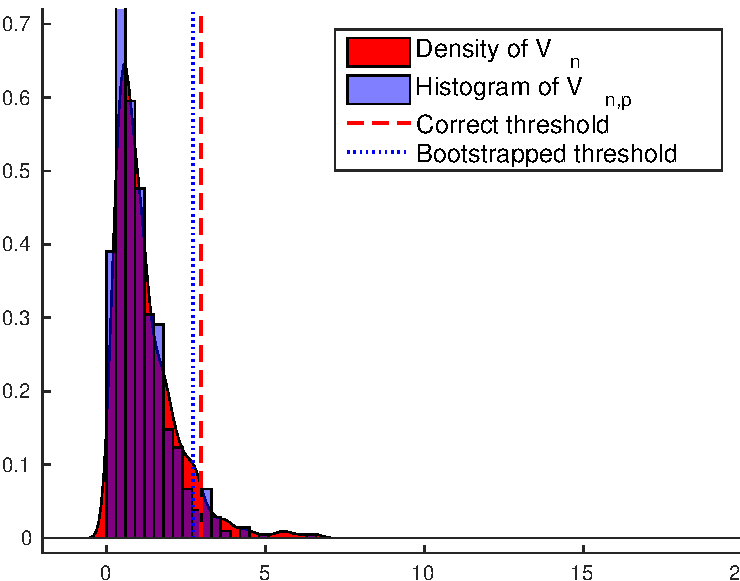
\includegraphics[width=0.55\textwidth]{../img/permfail_ecdf1.pdf}
\end{figure}
   
}

\section{Introduction}
\frame{
\frametitle{Back to the Difficult Problem}
\begin{columns}[c] 
    \column{.8\textwidth} 
    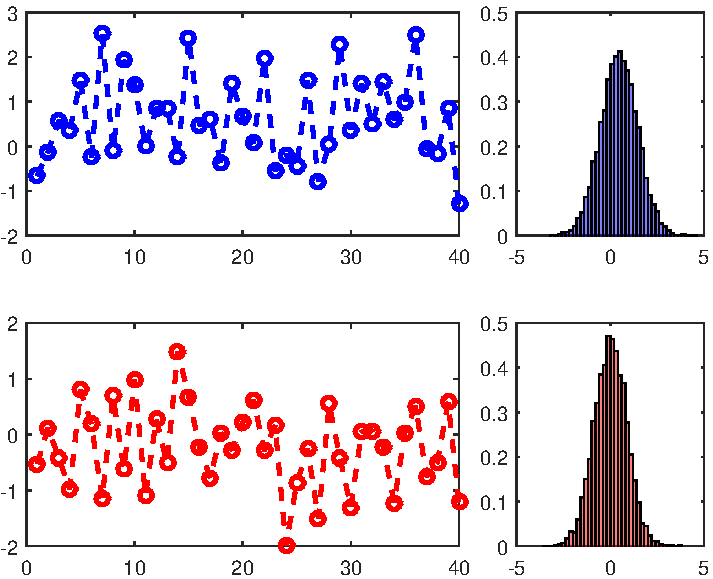
\includegraphics[height=0.8\textheight]{../img/introDep.pdf}
    \column{.2\textwidth}
    Is \\[1em] {\larger[5]$ \color{blue} P$} \\[1em] the same  distribution as  \\[1em]  {\larger[5]$\color{red} Q$} \\[1em] ?
    \end{columns}
}



\frame{
\frametitle{Memory of the Processes}
\begin{columns}[c] 
    \column{.6\textwidth} 
    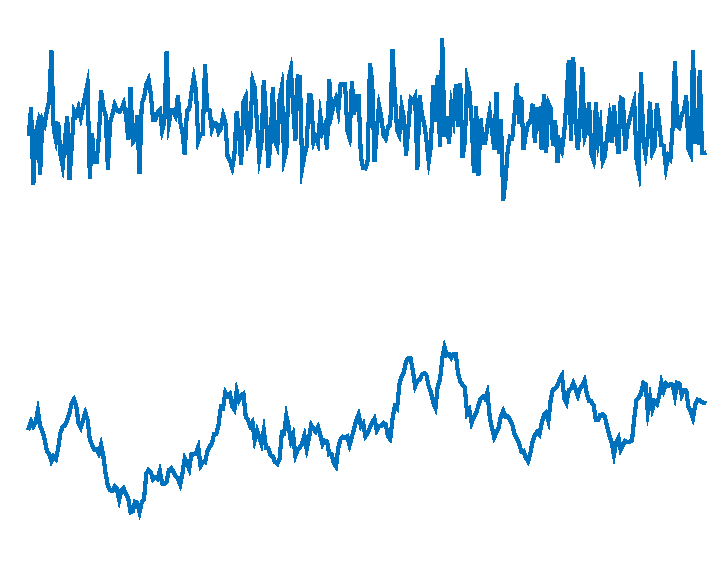
\includegraphics[width=\textwidth]{../img/processes.pdf}
    \column{.4\textwidth}
	{\larger[2]$$Q_t =  \mathbf{ \color{red} 0.14} Q_{t-1} + 0.98\epsilon_t$$ }
    Processes with different memory 
	{\larger[2]$$Z_t=   \mathbf{ \color{red} 0.97} Z_{t-1} +  0.22\epsilon_t.$$ }	
    \end{columns}
    \begin{alertblock}{The distribution of the $V$-statistics is primary driven by memory}
\end{alertblock}
}


\frame{\frametitle{Memory $0.1$}
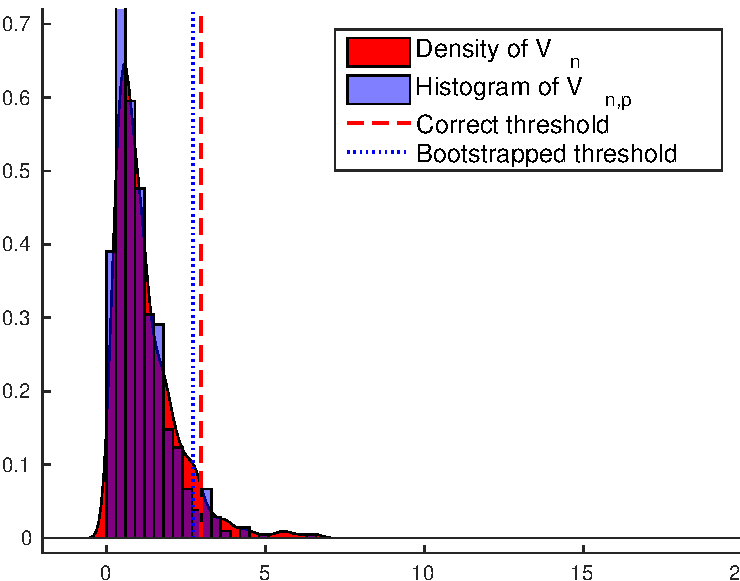
\includegraphics[width=0.9\textwidth, height=0.8\textheight]{../img/permfail_ecdf1.pdf} 
}

\frame{\frametitle{Memory $0.2$}
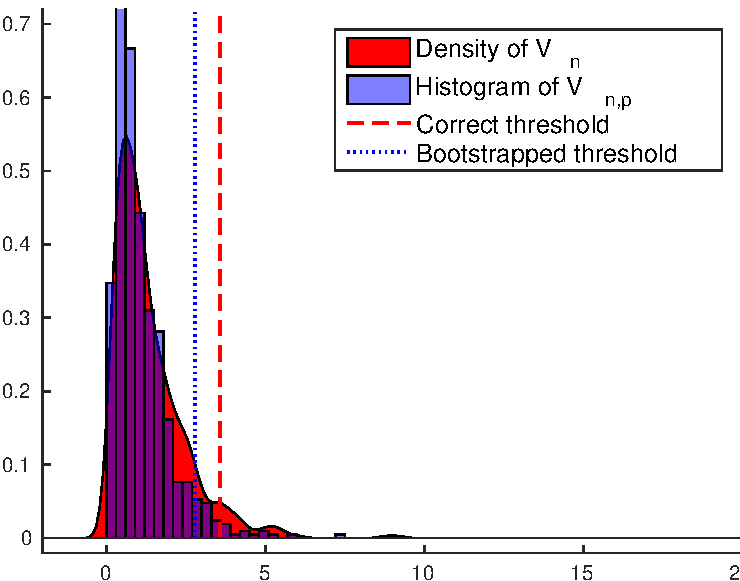
\includegraphics[width=0.9\textwidth, height=0.8\textheight]{../img/permfail_ecdf2.pdf} 
}

\frame{\frametitle{Memory $0.3$}
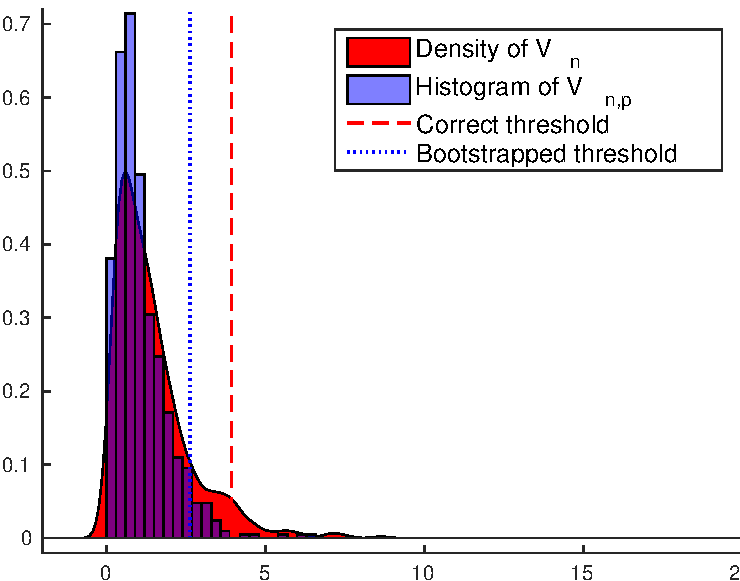
\includegraphics[width=0.9\textwidth, height=0.8\textheight]{../img/permfail_ecdf3.pdf} 
}

\frame{\frametitle{Memory $0.4$}
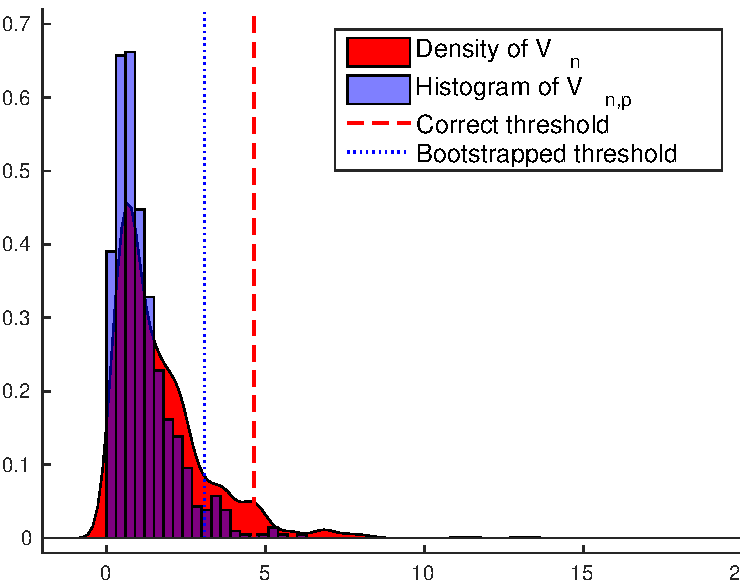
\includegraphics[width=0.9\textwidth, height=0.8\textheight]{../img/permfail_ecdf4.pdf} 
}

\frame{\frametitle{Memory $0.5$}
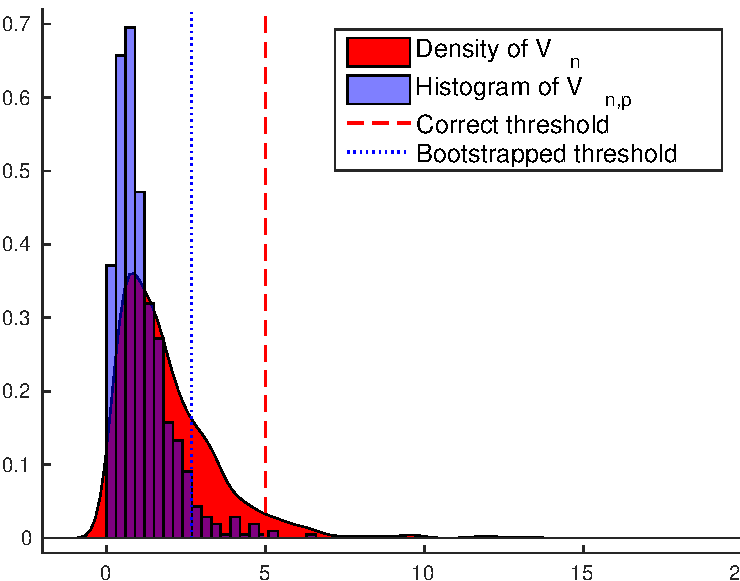
\includegraphics[width=0.9\textwidth, height=0.8\textheight]{../img/permfail_ecdf5.pdf} 
}

\frame{\frametitle{Memory $0.6$}
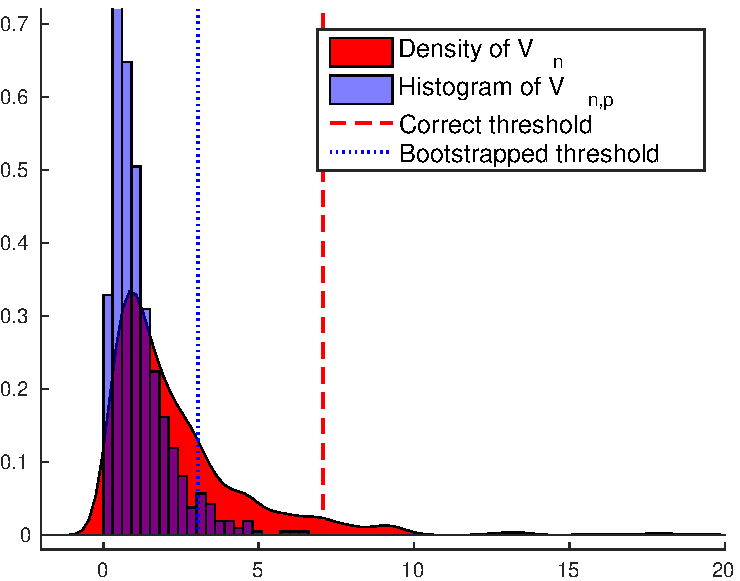
\includegraphics[width=0.9\textwidth, height=0.8\textheight]{../img/permfail_ecdf6.pdf} 
}

\frame{\frametitle{Memory $0.7$}
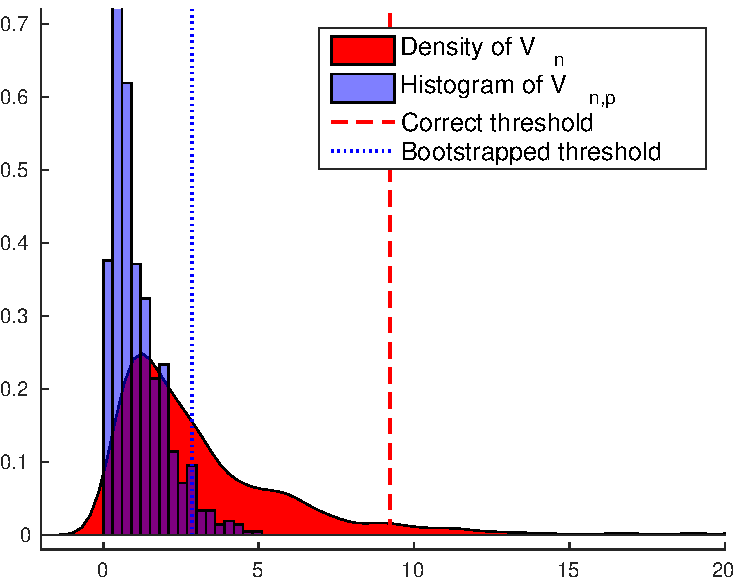
\includegraphics[width=0.9\textwidth, height=0.8\textheight]{../img/permfail_ecdf7.pdf} 
}

\frame{\frametitle{Memory $0.8$}
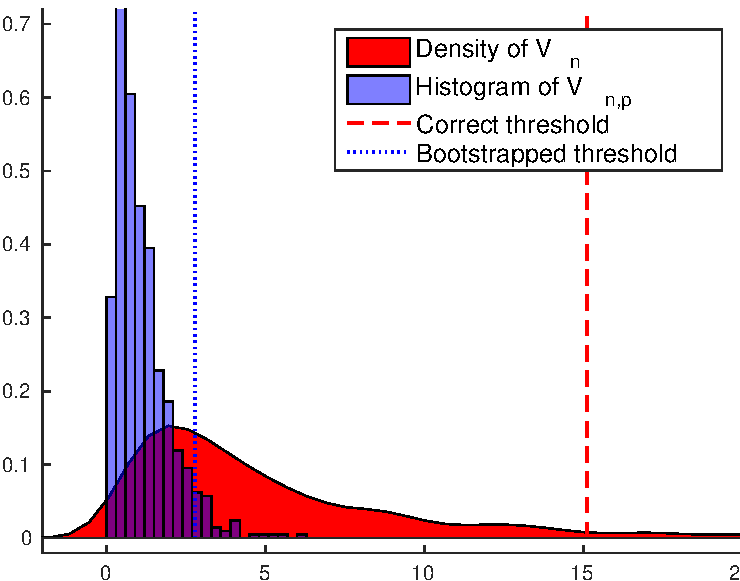
\includegraphics[width=0.9\textwidth, height=0.8\textheight]{../img/permfail_ecdf8.pdf} 
}


\newcommand{\kppmem}{\mathord{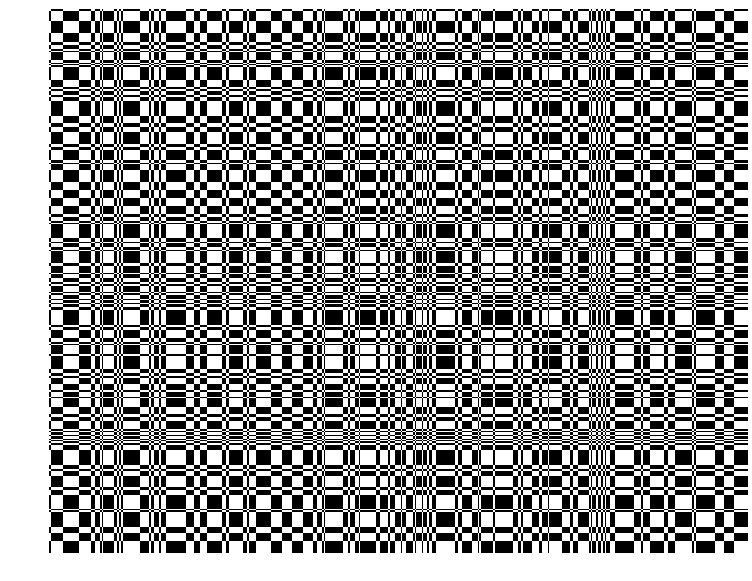
\includegraphics[height=2cm]{../img/KPPmem.pdf}}}
\newcommand{\kqqmem}{\mathord{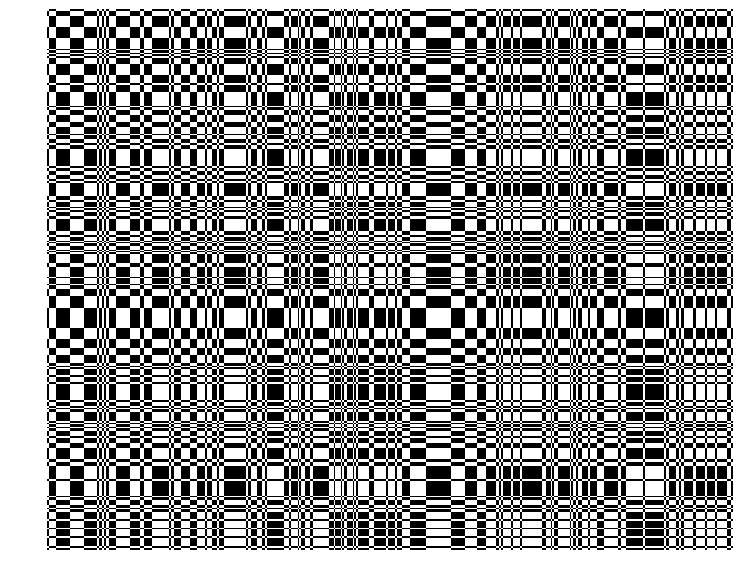
\includegraphics[height=2cm]{../img/KQQmem.pdf}}}
\newcommand{\kpqmem}{\mathord{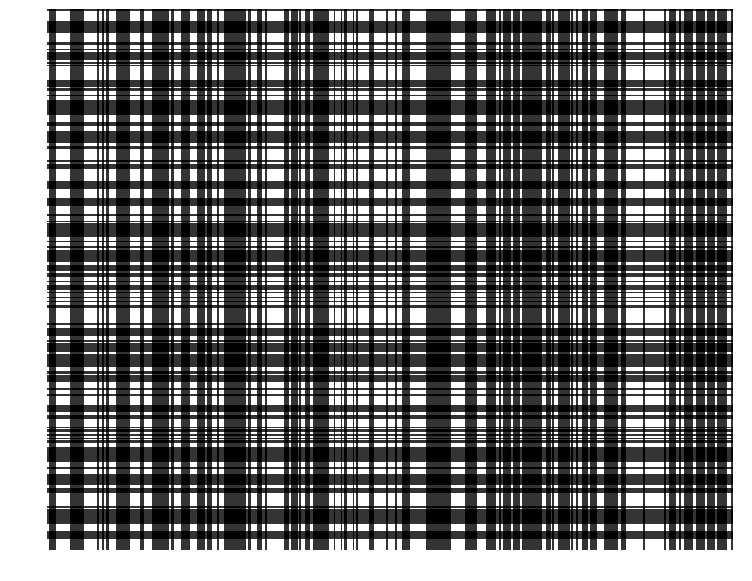
\includegraphics[height=2cm]{../img/KPQmem.pdf}}}

\frame{
\frametitle{Similarity for Random Processes}
\begin{align*}
K_{{\color{blue}P,P}}=
\begin{bmatrix}
	k( {\color{blue}X_1},{\color{blue}X_1)} &   \ldots & k({\color{blue}X_1},{\color{blue}X_n})\\
	\vdots &  \ddots & \vdots\\
	k({\color{blue}X_n},{\color{blue}X_1})  &  \ldots & k({\color{blue}X_n},{\color{blue}X_n})
\end{bmatrix} = 
\begin{matrix}
\kppmem
\end{matrix}
\\
K_{{\color{red}Q,Q}}=
\begin{bmatrix}
	k({\color{red}Y_1},{\color{red}Y_1)} &   \ldots & k({\color{red}Y_1},{\color{red}Y_n})\\
	\vdots &  \ddots & \vdots\\
	k({\color{red}Y_n},{\color{red}Y_1})  &  \ldots & k({\color{red}Y_n},{\color{red}Y_n})
\end{bmatrix}= 
\begin{matrix}
\kqqmem
\end{matrix}
\\
K_{{\color{blue}P,\color{red}Q}}=
\begin{bmatrix}
	k({\color{blue}X_1},{\color{red}Y_1}) &   \ldots & k({\color{blue}X_1},{\color{red}Y_n})\\
	\vdots &  \ddots & \vdots\\
	k({\color{blue}X_n},{\color{red}Y_1})  &  \ldots & k({\color{blue}X_n},{\color{red}Y_n})
\end{bmatrix}=
\begin{matrix}
\kpqmem
\end{matrix}
\end{align*}
}
\newcommand{\grammem}{\mathord{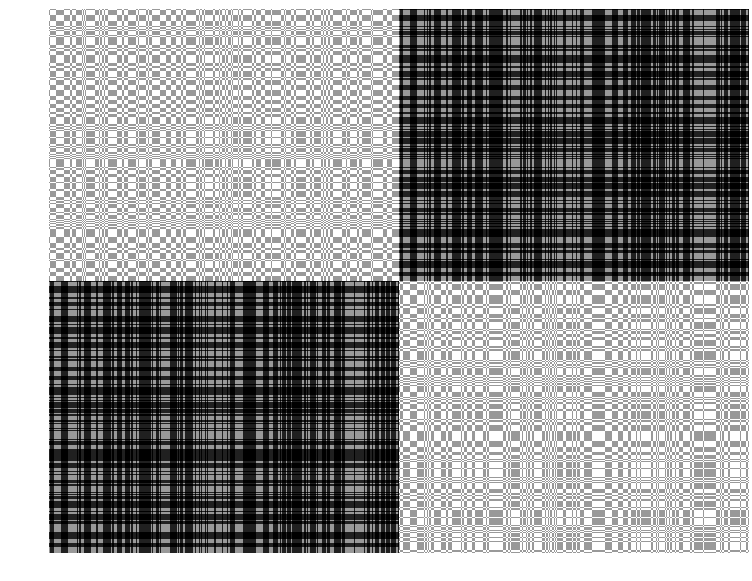
\includegraphics[height=2cm]{../img/Grammem.pdf}}}
\newcommand{\gramnmem}{\mathord{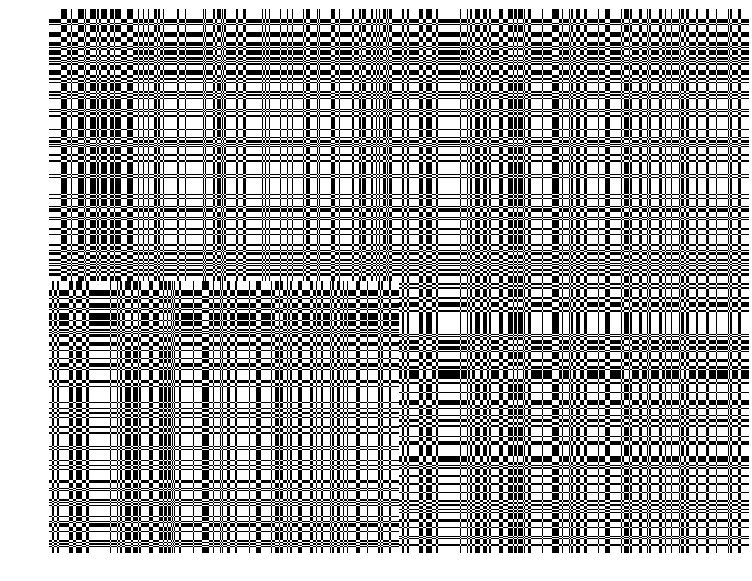
\includegraphics[height=2cm]{../img/Gramnmem.pdf}}}

\frame{
\frametitle{Gram Matrices}
\begin{align*}
{\color{blue} P} \neq {\color{red} Q} \quad \quad \Rightarrow 
\begin{bmatrix}
	K_{{\color{blue}P,P}}  &   K_{{\color{blue}P,\color{red}Q}}\\
	K_{{\color{red}Q},{\color{blue}P}}  &  K_{{\color{red}Q,Q}}
\end{bmatrix} = 
\begin{matrix}
\grammem
\end{matrix}
\end{align*}
\pause
\begin{align*}
{\color{blue} P }= {\color{red} Q} \quad \quad \Rightarrow 
\begin{bmatrix}
	K_{{\color{blue}P,P}}  &   K_{{\color{blue}P,\color{red}Q}}\\
	K_{{\color{red}Q},{\color{blue}P}}  &  K_{{\color{red}Q,Q}}
\end{bmatrix} = 
\begin{matrix}
\gramnmem
\end{matrix}
\end{align*}
}



\frame{
\frametitle{Permutation Test for Random Processes }
$$W= (-1,1,1,\dots,-1,-1,-1)$$
\begin{align*}
&{\begin{bmatrix}
	K_{{\color{blue}P,P}}  &   K_{{\color{blue}P,\color{red}Q}}\\
	K_{{\color{red}Q},{\color{blue}P}}  &  K_{{\color{red}Q,Q}}
\end{bmatrix} } & \odot
&\begin{bmatrix}
\Scale[2] {W \trans{W}}
\end{bmatrix} &= 
&\begin{bmatrix}
\Scale[2] ?
\end{bmatrix} \\
&\begin{matrix}
\grammem
\end{matrix} &\odot
&\begin{matrix}
\kpp
\end{matrix} &=
&\begin{matrix} 
\gramn
\end{matrix} \\
&\begin{matrix}
\gramnmem
\end{matrix} &\odot
&\begin{matrix}
\kpp
\end{matrix} &=
&\begin{matrix} 
\gramn
\end{matrix} \\
\end{align*}

}

\frame{
\frametitle{If ${\color{blue} P} = {\color{red} Q}$ Permutation Approach Fails}
\begin{columns}[c] 
  \column{.5\textwidth} 
  \begin{figure}
  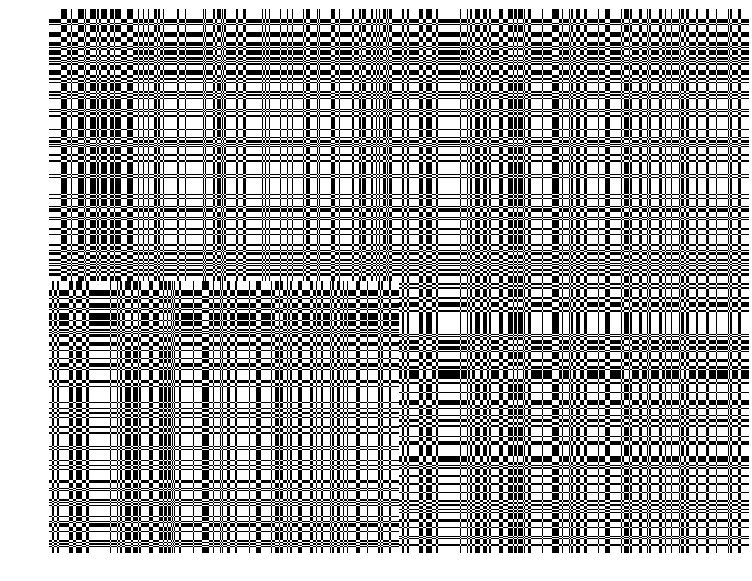
\includegraphics[height=4.5cm]{../img/Gramnmem.pdf}
  \caption*{The actual matrix}
  \end{figure} 
  \column{.5\textwidth}
  \begin{figure}
  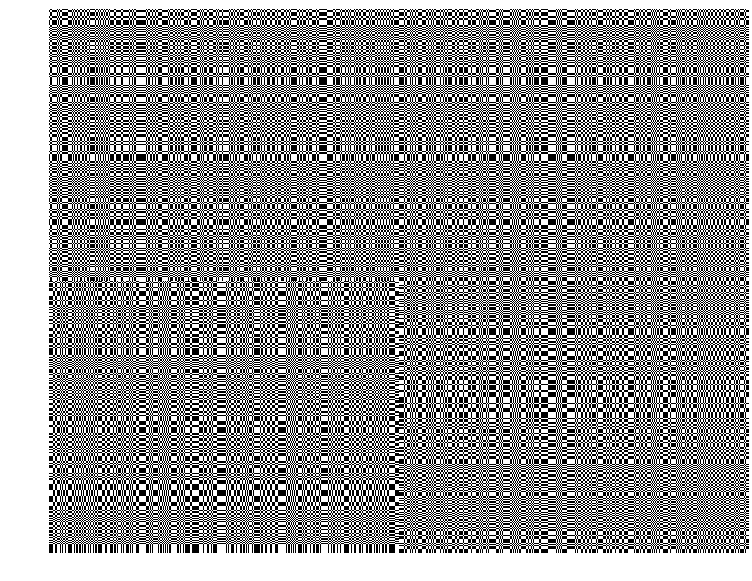
\includegraphics[height=4.5cm]{../img/Gramn.pdf}
  \caption*{Matrix generated via permutation}
  \end{figure}	
\end{columns}
}

%\frame{\frametitle{Permutation bootstrap approximation of ${\color{PineGreen} V}$}
%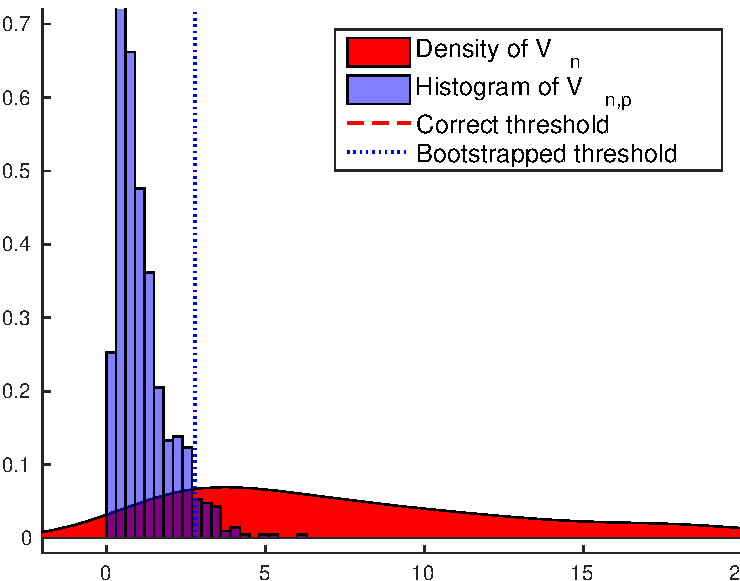
\includegraphics[width=0.9\textwidth, height=0.8\textheight]{../img/permfail_ecdf9.pdf} 
%}
\section{Wild Bootstrap}



\newcommand{\wildAlt}{\mathord{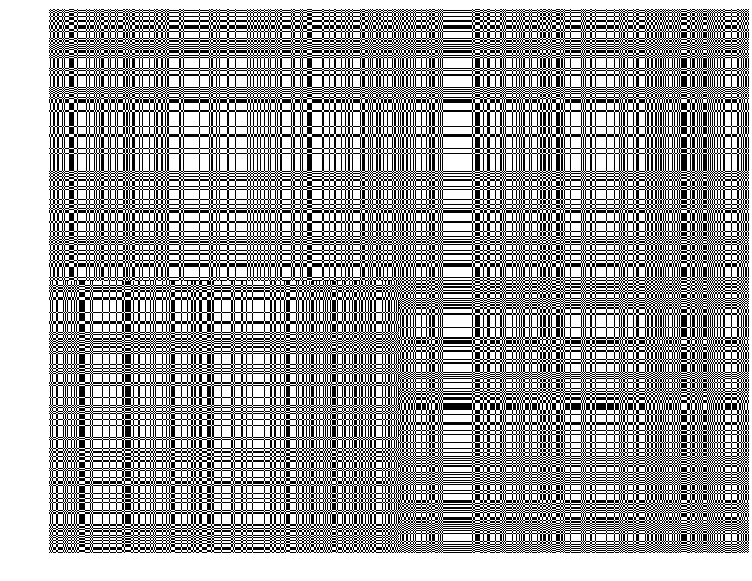
\includegraphics[height=2cm]{../img/wildAlt.pdf}}}
\newcommand{\wildNull}{\mathord{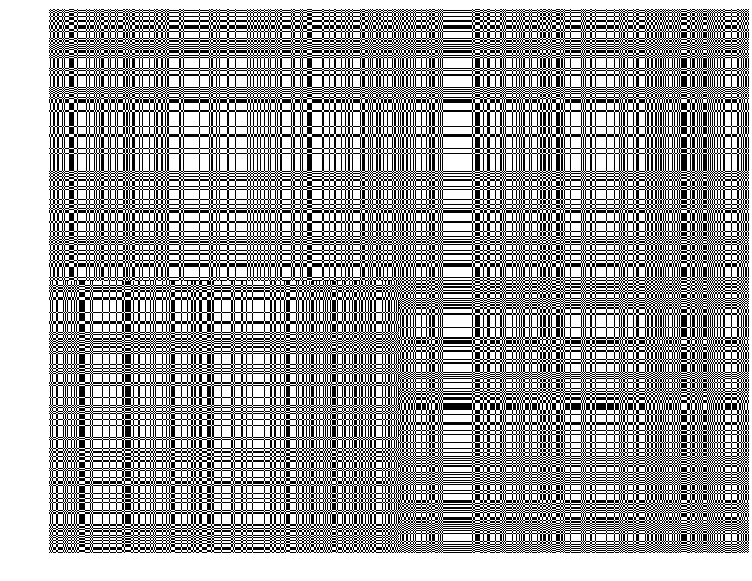
\includegraphics[height=2cm]{../img/wildNull.pdf}}}
\newcommand{\wildMatrix}{\mathord{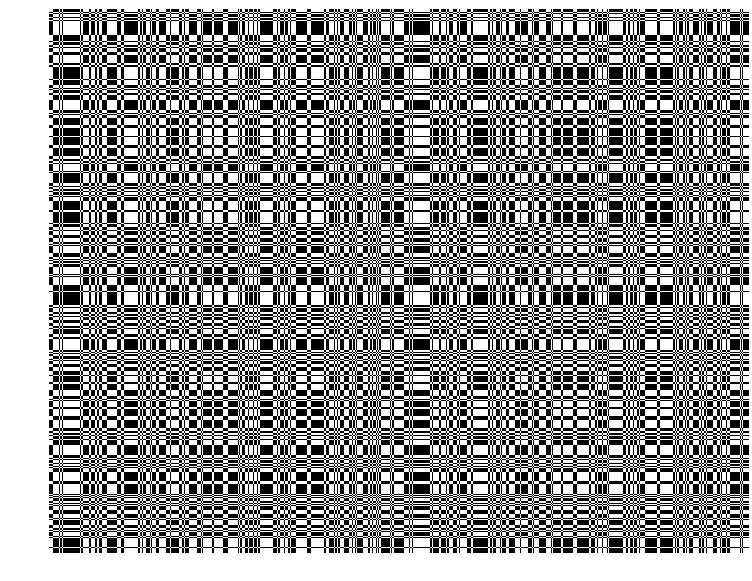
\includegraphics[height=2cm]{../img/wildmatrix.pdf}}}
\frame{
\frametitle{Wild Bootstrap}
\begin{center}
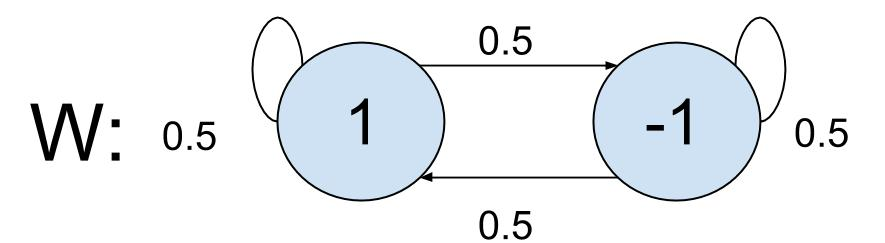
\includegraphics[height=1.5cm]{../img/markowChain.jpg}
\end{center}
\begin{align*}
&{\begin{bmatrix}
	K_{{\color{blue}P,P}}  &   K_{{\color{blue}P,\color{red}Q}}\\
	K_{{\color{red}Q},{\color{blue}P}}  &  K_{{\color{red}Q,Q}}
\end{bmatrix} } & \odot
&{\begin{bmatrix}
	W\trans{W}  &  -W\trans{W}\\
	-W\trans{W}  &  W\trans{W}
\end{bmatrix} }&= 
&\begin{bmatrix}
\Scale[2] ?
\end{bmatrix} \\
&\begin{matrix}
\grammem
\end{matrix} &\odot
&\begin{matrix}
\wildMatrix
\end{matrix} &=
&\begin{matrix} 
\wildAlt
\end{matrix} \\
&\begin{matrix}
\gramnmem
\end{matrix} &\odot
&\begin{matrix}
\wildMatrix
\end{matrix} &=
&\begin{matrix} 
\wildNull
\end{matrix} \\
\end{align*}

}



\frame{
\frametitle{If ${\color{blue} P} = {\color{red} Q}$ the Wild Bootstrap Approach Works!}
\begin{columns}[c] 
  \column{.5\textwidth} 
  \begin{figure}
  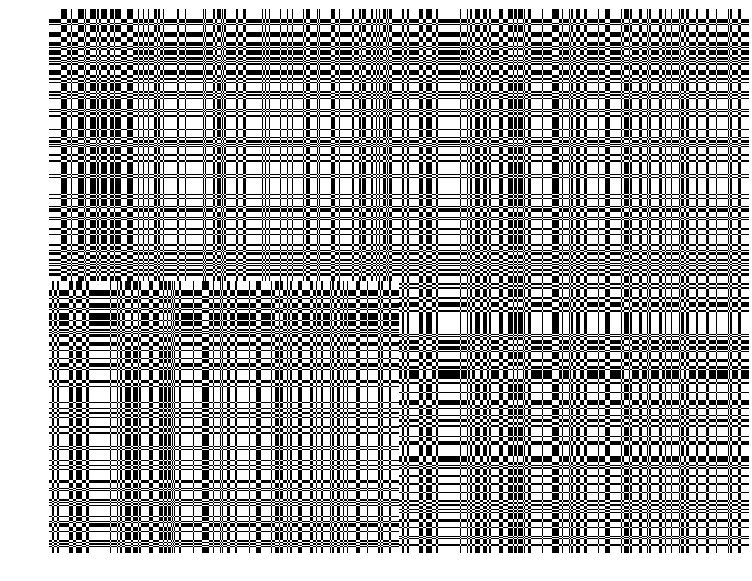
\includegraphics[height=4cm]{../img/Gramnmem.pdf}
  \caption*{The actual matrix}
  \end{figure} 
  \column{.5\textwidth}
  \begin{figure}
  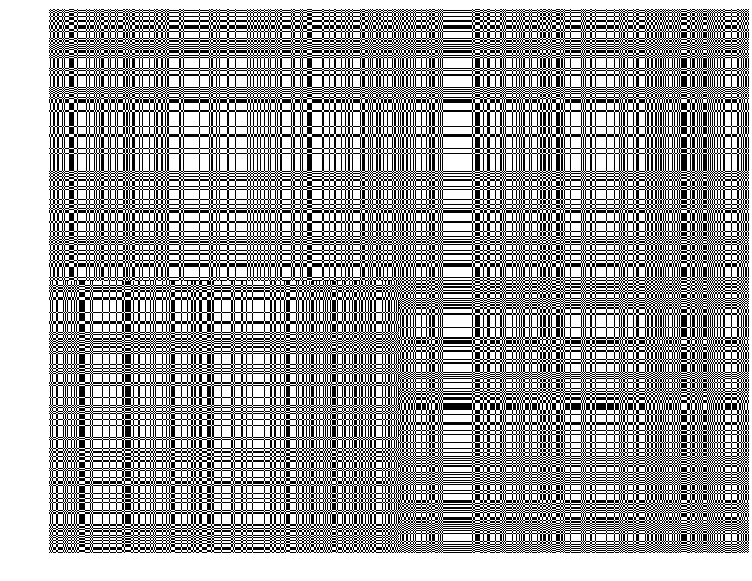
\includegraphics[height=4cm]{../img/wildNull.pdf}
  \caption*{Matrix generated via \bf{wild bootstrap}}
  \end{figure}	
\end{columns}
}

\frame{
\frametitle{Estimation of $V_n$ via the Wild Bootstrap}
\begin{center}
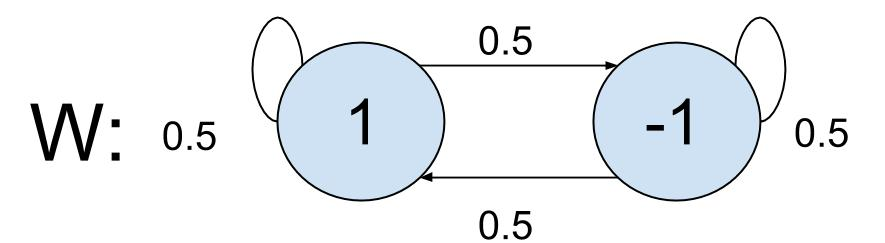
\includegraphics[height=1.5cm]{../img/markowChain.jpg}
\end{center}

\begin{align*}
\Scale[1.5]{V_{n,w}=\overline{
\begin{bmatrix}
	K_{{\color{blue}P,P}}  &   K_{{\color{blue}P,\color{red}Q}}\\
	K_{{\color{red}Q},{\color{blue}P}}  &  K_{{\color{red}Q,Q}}
\end{bmatrix}   \odot
\begin{bmatrix}
	W\trans{W}  &  -W\trans{W}\\
	-W\trans{W}  &  W\trans{W}
\end{bmatrix} }}
\end{align*}


}

\frame{\frametitle{Memory $0.1$}
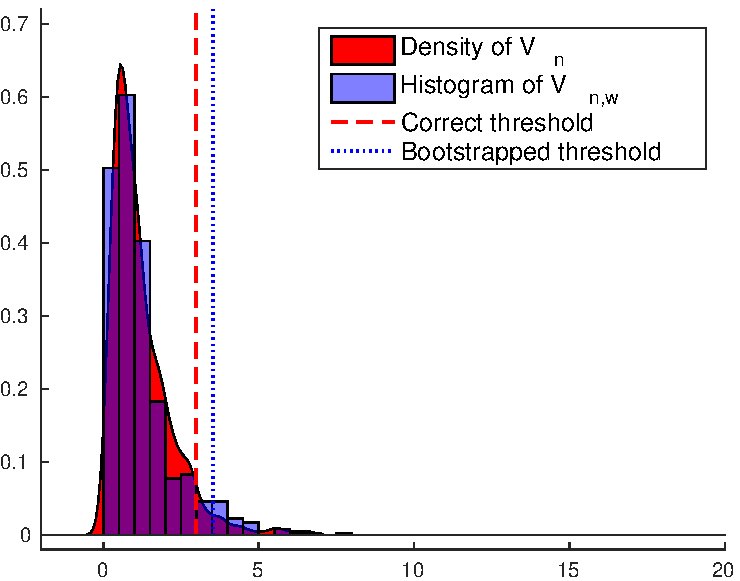
\includegraphics[width=0.9\textwidth, height=0.8\textheight]{../img/wild_ecdf1.pdf} 
}

\frame{\frametitle{Memory $0.2$}
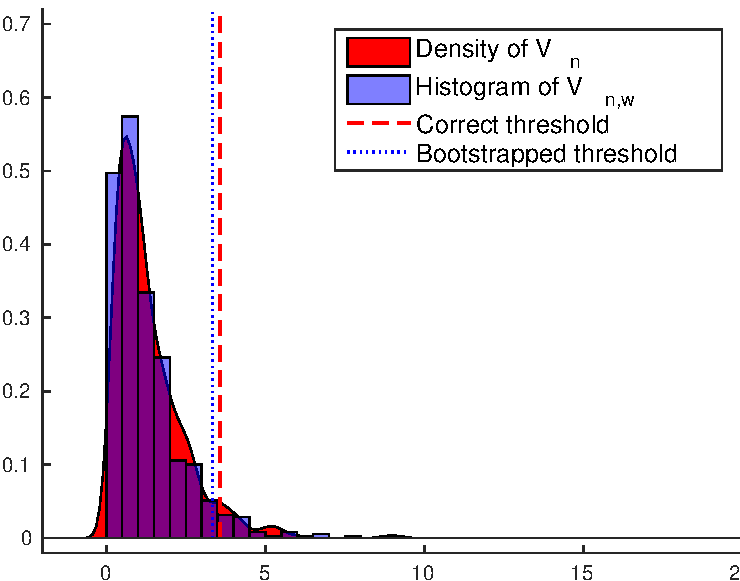
\includegraphics[width=0.9\textwidth, height=0.8\textheight]{../img/wild_ecdf2.pdf} 
}

\frame{\frametitle{Memory $0.3$}
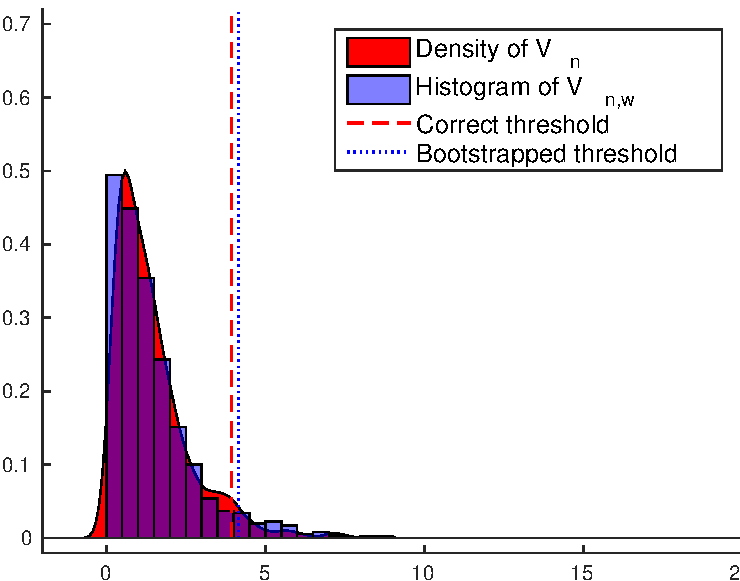
\includegraphics[width=0.9\textwidth, height=0.8\textheight]{../img/wild_ecdf3.pdf} 
}

\frame{\frametitle{Memory $0.4$}
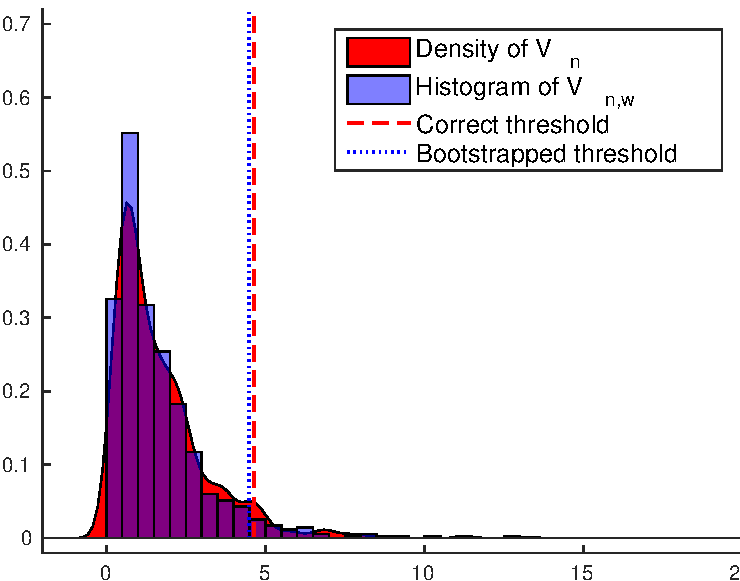
\includegraphics[width=0.9\textwidth, height=0.8\textheight]{../img/wild_ecdf4.pdf} 
}

\frame{\frametitle{Memory $0.5$}
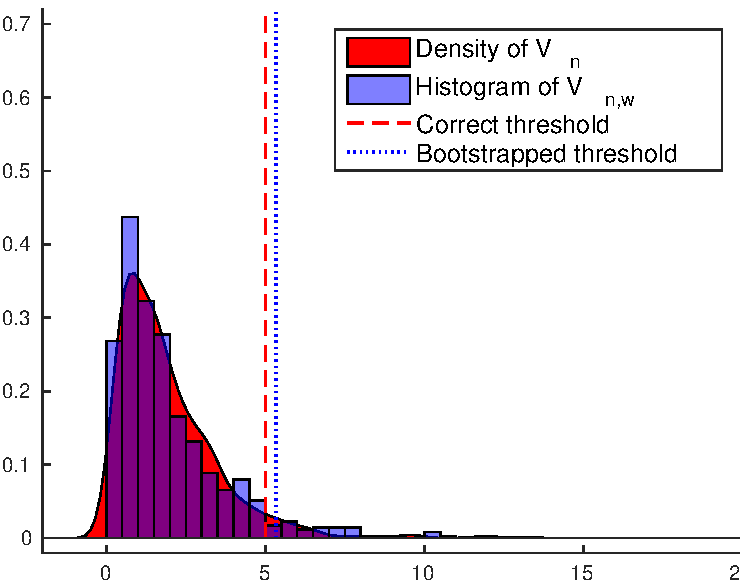
\includegraphics[width=0.9\textwidth, height=0.8\textheight]{../img/wild_ecdf5.pdf} 
}

\frame{\frametitle{Memory $0.6$}
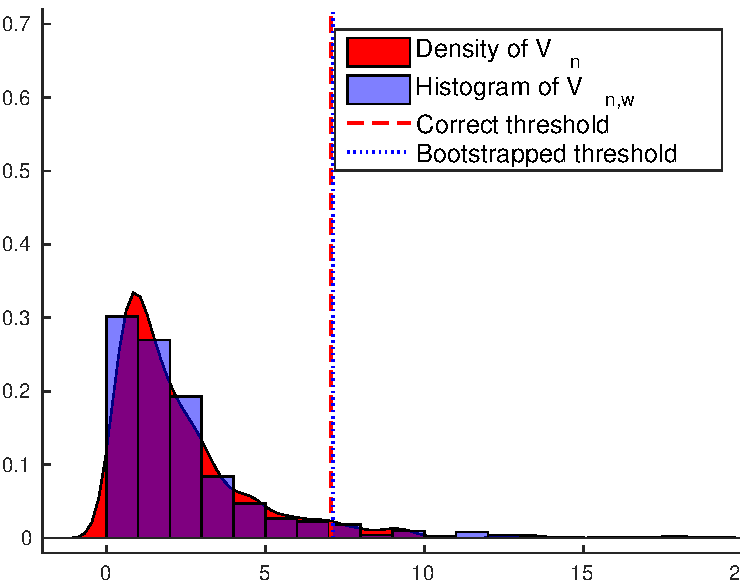
\includegraphics[width=0.9\textwidth, height=0.8\textheight]{../img/wild_ecdf6.pdf} 
}

\frame{\frametitle{Memory $0.7$}
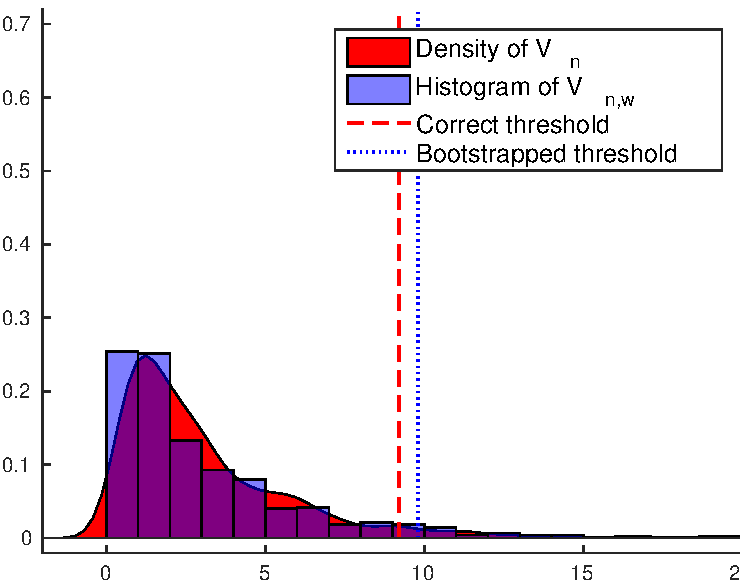
\includegraphics[width=0.9\textwidth, height=0.8\textheight]{../img/wild_ecdf7.pdf} 
}


\frame{\frametitle{Memory $0.8$}
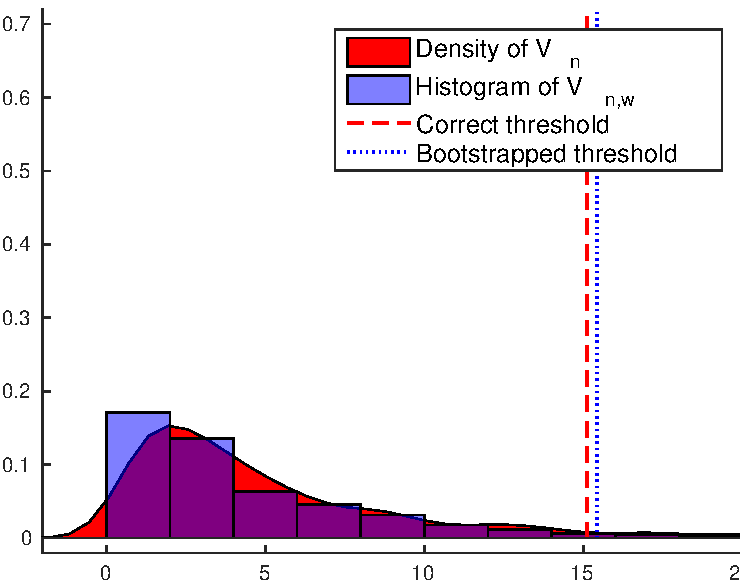
\includegraphics[width=0.9\textwidth, height=0.8\textheight]{../img/wild_ecdf8.pdf} 
}
%
%\frame{\frametitle{Wild Bootstrap Approximation - ${\color{Plum} V_{b}}$ distribution}
%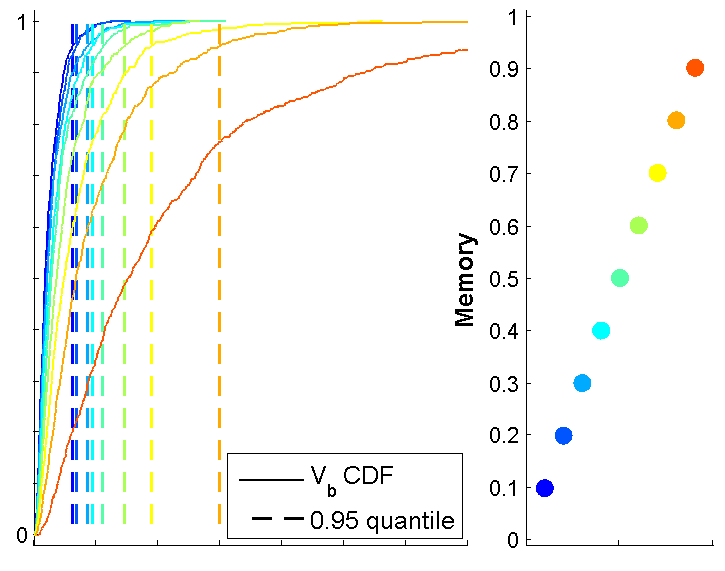
\includegraphics[width=0.9\textwidth, height=0.8\textheight]{../img/wild_ecdf9.pdf} 
%}

 
\frame{
\frametitle{MCMC M.D. Experiment}


\begin{columns}[c] 
    \column{.4\textwidth} 
    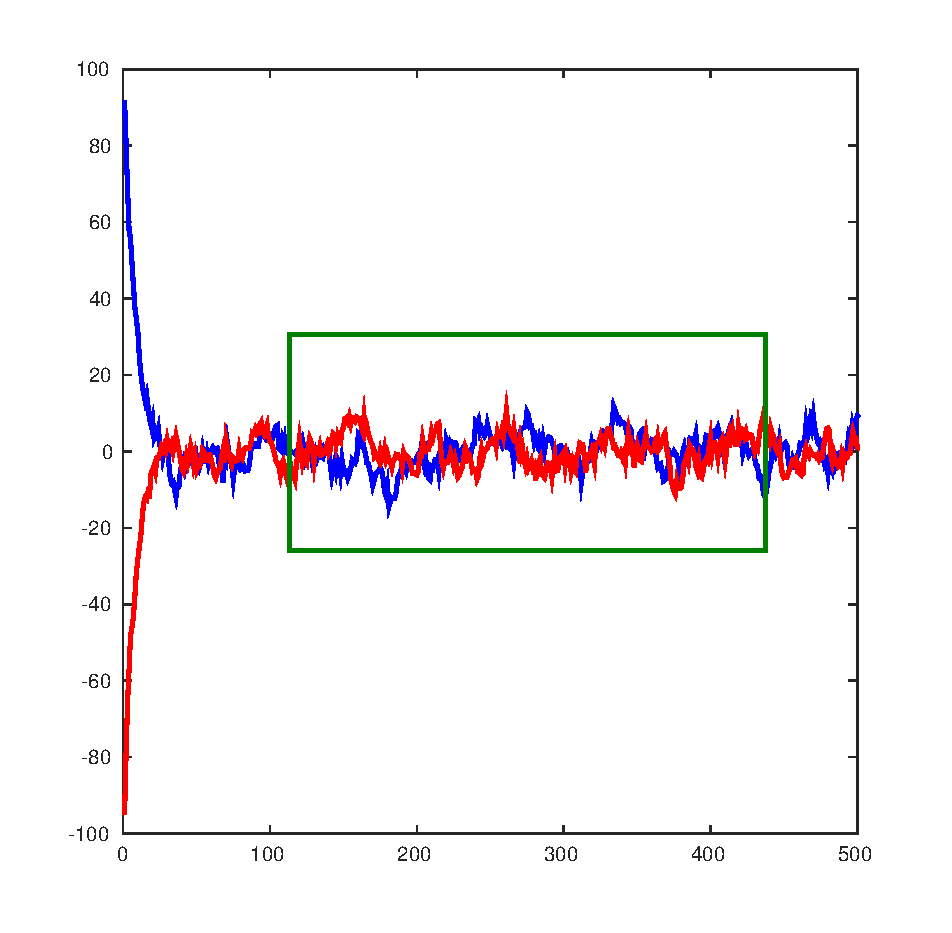
\includegraphics[height=0.6\textheight]{../img/mcmc.pdf}
    \column{.6\textwidth}
    Is  {\larger[3]$ \color{blue} P$}  the same  distribution as    {\larger[3]$\color{red} Q$}  ?
\begin{table}	
	\begin{tabular}{ l | c  }
  \hline                       
  Test - MMD                  &  Type one error  \\  
    \hline   
  Permutation        & 68 \%   \\
    \hline   
  Wild Bootstrap    & 6 \%   \\
  \hline  
\end{tabular}

\end{table}    
    
    \end{columns}


}


\frame{
\frametitle{Indie Pop Group Predicts the Volume of the Dow Jones!}
\begin{center}
\begin{columns}[c] 
    \column{.5\textwidth} 
    \begin{center}
    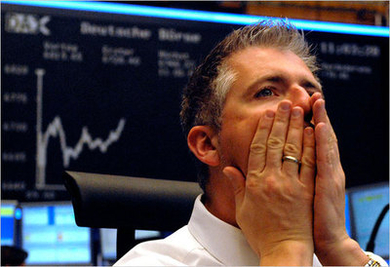
\includegraphics[width=0.4\textheight]{../img/sad-guys-on-trading-floors.jpg}
	\end{center}   
    \column{.5\textwidth}
    \begin{center}
    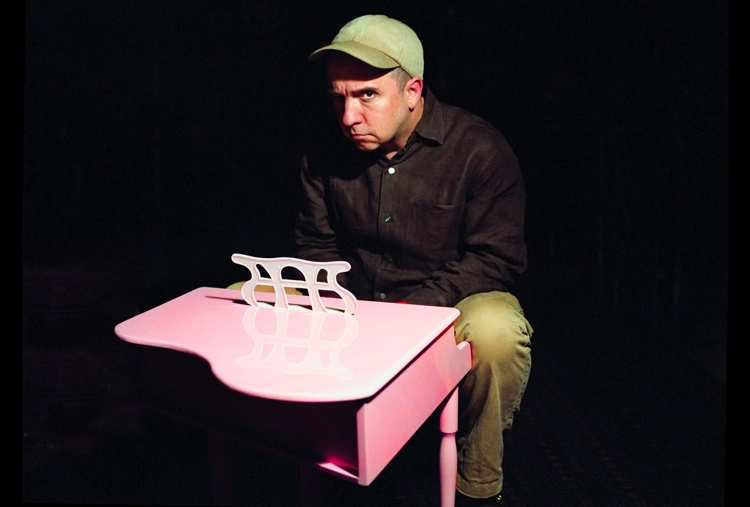
\includegraphics[width=0.4\textheight]{../img/strange_powers_01.jpg} 
	\end{center}
\end{columns}
\end{center}
\pause 
\begin{table}
\begin{tabular}{ l | c | c| c }
  \hline                       
  Test                   & p-value& Dependent   \\  
    \hline   
  Permutation HSIC       & 0.003  & Yes ! \\
    \hline   
  \pause 
  Wild Bootstrap HSIC    & 0.231  & \colorbox{red}{No} \\
  \hline  
\end{tabular}

\end{table}
}
 

\end{document}


